\subsection{Diagonalization and Power Sets}

\begin{theorem} \label{thm:cantor-power-set-theorem} \hlt{Cantor's Theorem}\\
Let $X$ be a set. No function $f:X\to\mathcal{P}(X)$ is surjective; hence $X\not\sim_{\#}\mathcal{P}(X)$.
\begin{proof}
Fix $f:X\to\mathcal{P}(X)$ and set $D_f\defeq\{x\in X:x\notin f(x)\}$. Then $D_f\subseteq X$, so $D_f\in\mathcal{P}(X)$.\\
If $a\in X$ and $D_f=f(a)$, then $a\in D_f\Longleftrightarrow a\in f(a)$, contrary to $a\in D_f\Longleftrightarrow a\notin f(a)$.\\
Hence $(\forall a\in X)\,D_f\neq f(a)$, so $D_f\notin f(X)$ and $f$ is not surjective. Since a bijection must be surjective, $X\not\sim_{\#}\mathcal{P}(X)$.\\
\hlt{Structural Commentary}: The diagonal subset differs from each image set at its own indexing element.\\
\hlt{Key Insight}: Diagonal self-membership forces $(\forall a\in X)\,D_f\neq f(a)$.
\end{proof}
\end{theorem}

\begin{proposition} \label{prop:binary-sequences-model-power-set} \hlt{Binary Sequences Model a Power Set}\\
Let $A\defeq\{0,1\}^{\N}$. Define $\Phi:A\to\mathcal{P}(\N)$ by $\Phi(s)\defeq\{n\in\N:s(n)=1\}$. Then $\Phi$ is bijective.
\begin{proof}
For $E\subseteq\N$, define $\chi_E:\N\to\{0,1\}$ by $\chi_E(n)\defeq1$ when $n\in E$ and $\chi_E(n)\defeq0$ otherwise. Define $\Psi:\mathcal{P}(\N)\to A$ by $\Psi(E)\defeq\chi_E$.\\
If $E\subseteq\N$ and $n\in\N$, then $n\in\Phi(\Psi(E))\Longleftrightarrow\chi_E(n)=1\Longleftrightarrow n\in E$. Hence $\Phi(\Psi(E))=E$ by Assumption \ref{assump:set-extensionality}.\\
If $s\in A$ and $n\in\N$, then $\chi_{\Phi(s)}(n)=1\Longleftrightarrow s(n)=1$. Both values lie in $\{0,1\}$, so $\chi_{\Phi(s)}(n)=s(n)$. Thus $(\forall n\in\N)\,\chi_{\Phi(s)}(n)=s(n)$.\\
Hence $\Psi(\Phi(s))=s$ by Assumption \ref{assump:function-extensionality}. The maps $\Phi$ and $\Psi$ are inverse, so $\Phi$ is bijective by Theorem \ref{thm:bijective-iff-invertible-function}.\\
\hlt{Structural Commentary}: Characteristic functions construct a two-sided inverse to the subset-extraction map.\\
\hlt{Key Insight}: A membership bit records exactly one subset decision.
\end{proof}
\end{proposition}

\begin{theorem} \label{thm:binary-sequences-uncountable} \hlt{Binary Sequences Are Uncountable}\\
Let $A\defeq\{0,1\}^{\N}$. Then $A$ is uncountable.
\begin{proof} Define $j:\N\to\mathcal{P}(\N)$ by $j(n)\defeq\{n\}$, and define $\Phi:A\to\mathcal{P}(\N)$ by $\Phi(s)\defeq\{n\in\N:s(n)=1\}$.\\
The map $j$ is injective because $j(m)=j(n)$ implies $m=n$. The map $\Phi$ is bijective by Proposition \ref{prop:binary-sequences-model-power-set}, so $\Phi^{-1}\circ j:\N\to A$ is injective.\\
If $A$ were finite, choose $m\in\N_0$ and a bijection $q:A\to J_m$.\\
Then $q\circ\Phi^{-1}\circ j:\N\to J_m$ would be injective. No such injection exists by Proposition \ref{prop:natural-numbers-do-not-inject-into-finite-sets}(i), a contradiction.\\
Thus $A$ is not finite. Suppose $A$ were countable. Choose a bijection $e:\N\to A$, and write $s_n\defeq e(n)$.\\
Define $s:\N\to\{0,1\}$ by $s(k)\defeq1-s_k(k)$. Then $s\in A$ and $(\forall n\in\N)\,s(n)\neq s_n(n)$, so $(\forall n\in\N)\,s\neq e(n)$.\\
This contradicts the surjectivity of $e$. Hence $A$ is neither finite nor countable, so it is uncountable.\\
\hlt{Structural Commentary}: An embedded copy of $\N$ excludes finiteness; a diagonal flip excludes enumerability.\\
\hlt{Key Insight}: The $n$th flipped bit separates the new sequence from row $n$.
\end{proof}
\end{theorem}

\begin{illustrationfigure}[H]
  \centering
  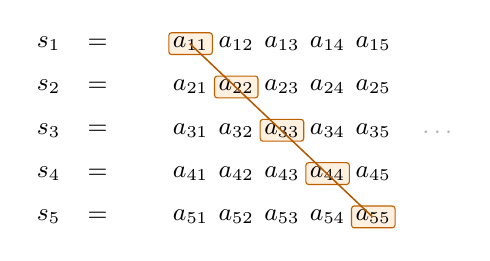
\begin{tikzpicture}[
  every node/.style={font=\small},
  digit/.style={font=\small},
  diagonal/.style={draw=orange!75!black, fill=orange!12, rounded corners=1pt, inner sep=1.5pt},
  guide/.style={orange!70!black, line width=0.55pt}
]
  \foreach \row/\name in {1/s_1,2/s_2,3/s_3,4/s_4,5/s_5} {
    \node[anchor=east] at (0,-0.55*\row) {$\name$};
    \node at (0.35,-0.55*\row) {$=$};
  }

  \foreach \row in {1,...,5} {
    \foreach \col in {1,...,5} {
      \node[digit] at (0.95+0.58*\col,-0.55*\row) {$a_{\row\col}$};
    }
  }

  \foreach \row in {1,...,5} {
    \node[diagonal] at (0.95+0.58*\row,-0.55*\row) {$a_{\row\row}$};
  }
  \draw[guide] (1.52,-0.55) -- (3.84,-2.75);

  \node[anchor=west, gray!60] at (4.35,-1.68) {$\cdots$};
\end{tikzpicture}

  \caption{Boxed entries $a_{nn}=s_n(n)$ whose bit flips define a sequence distinct from every listed row.}
  \label{fig:cantor-diagonal-binary-sequences}
\end{illustrationfigure}

Figure \ref{fig:cantor-diagonal-binary-sequences} marks the diagonal entries used in Theorem \ref{thm:binary-sequences-uncountable}.\\
Flipping the $n$th boxed bit forces $s(n)\neq s_n(n)$, so the constructed sequence cannot equal row $n$.
